\scanpage{98}
\mspage{48}
\margin{Case of a strict normalization morphism.}
From this viewpoint, one sees that in the case where \inserted{$S'\simeq S$,} $I'\xrightarrow{\sim}I\amalg\widetilde J$, one obtains $G'$ from $G\deleted{\unsure{'}}$ by giving oneself the set $C$ of \deleted{\unsure{arrows|feet}}\inserted{edges (ordinary)} of $G\deleted{\unsure{'}}$ ``that one wants to remove'' (\inserted{$\widetilde C$ is the} complement of $I'$ in $(\widehat I'\longrightarrow\widehat I)$ by taking a point on each edge $\in C$, and by ``cutting'' the edge at this point with a snip of the scissors (i.e taking the cutting of $X$ along the finite subset marked on $X$)

% Two opening parentheses precede the complement expression, but only one closing parenthesis is visible there.
\figure{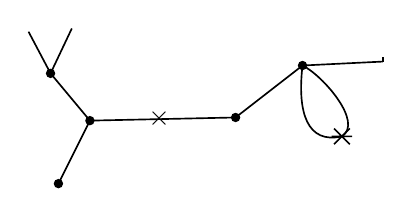
\begin{tikzpicture}[x=1cm,y=1cm,line width=.6pt]
\coordinate (a) at (0,0);
\coordinate (b) at (-.5,.6);
\coordinate (c) at (-.4,-.8);
\coordinate (d) at (1.85,.04);
\coordinate (e) at (2.7,.7);
\draw (b)--(a)--(c) (a)--(d)--(e);
\draw (b)--(-.78,1.13) (b)--(-.23,1.17) (e)--(3.72,.75);
\draw (3.72,.75)--(3.72,.81);
\draw (e) .. controls (2.63,.1) and (2.76,-.3) .. (3.2,-.2)
  .. controls (3.48,-.02) and (2.95,.58) .. (e);
\foreach \p in {a,b,c,d,e} {\fill (\p) circle (1.7pt);}
\node at (.88,.02) {$\times$};
\draw (3.10,-.30)--(3.30,-.10) (3.10,-.10)--(3.30,-.30) (3.07,-.2)--(3.33,-.2);
\end{tikzpicture}}
gives
\figure{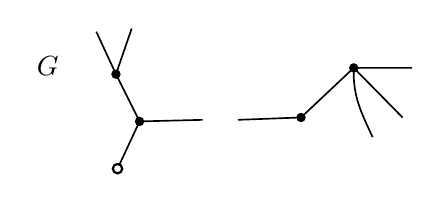
\begin{tikzpicture}[x=1cm,y=1cm,line width=.6pt]
\node[left] at (-.9,.7) {$G$};
\coordinate (a) at (0,0);
\coordinate (b) at (-.3,.6);
\coordinate (c) at (-.28,-.6);
\coordinate (d) at (2.05,.05);
\coordinate (e) at (2.72,.68);
\draw (b)--(a)--(c) (a)--(.8,.02) (b)--(-.55,1.14) (b)--(-.1,1.18);
\draw (1.25,.02)--(d)--(e) (e)--(3.46,.68) (e)--(3.34,.05);
\draw (e) to[out=-92,in=115] (2.96,-.2);
\foreach \p in {a,b,d,e} {\fill (\p) circle (1.7pt);}
% The lower-left endpoint has a visible open centre in this drawing.
\draw[line width=.8pt,fill=white] (c) circle (1.7pt);
\end{tikzpicture}}

One finds a new graph with flattened branches (which has a chance of being disconnected, even if $G$ was connected \unsure{\}|!} — even if $G$ had no flattened branches, it tends to have some\ldots).
\margin{In the reverse direction, is derived from $G'$ by giving oneself an involution without fixed points \unsure{in|of} the set of its ``flattened'' branches, which makes it possible to ``glue together'' these by their ends.}
If moreover one \deleted{\unsure{f}} replaces $G'$ by a subgraph derived from $G'$ by removing certain flattened branches, and by taking a union of connected components of what remains (by \deleted{\unsure{preserving|conversely})} \inserted{moreover} it is
% The baseline en survives; the raised en is separate. The old closing parenthesis is crossed out.
\margin{97}
